\chapter{Rotazione degli assi in 3D}

In questa lezione studieremo come legare il moto degli assi mobili solidali al corpo a quelli fissi e viceversa.

Un primo metodo, più rudimentale ma valido nelle applicazioni, è dato dagli angoli di Cardano.

\begin{definition}{}[Angoli di Cardano]
Gli angoli di Cardano $\theta$, $\varphi$, $\psi$ sono i tre angoli, rispetto a un riferimento fisso, illustrati in figura.
\end{definition}
\begin{center}
\begin{minipage}{0.45\textwidth}
\centering
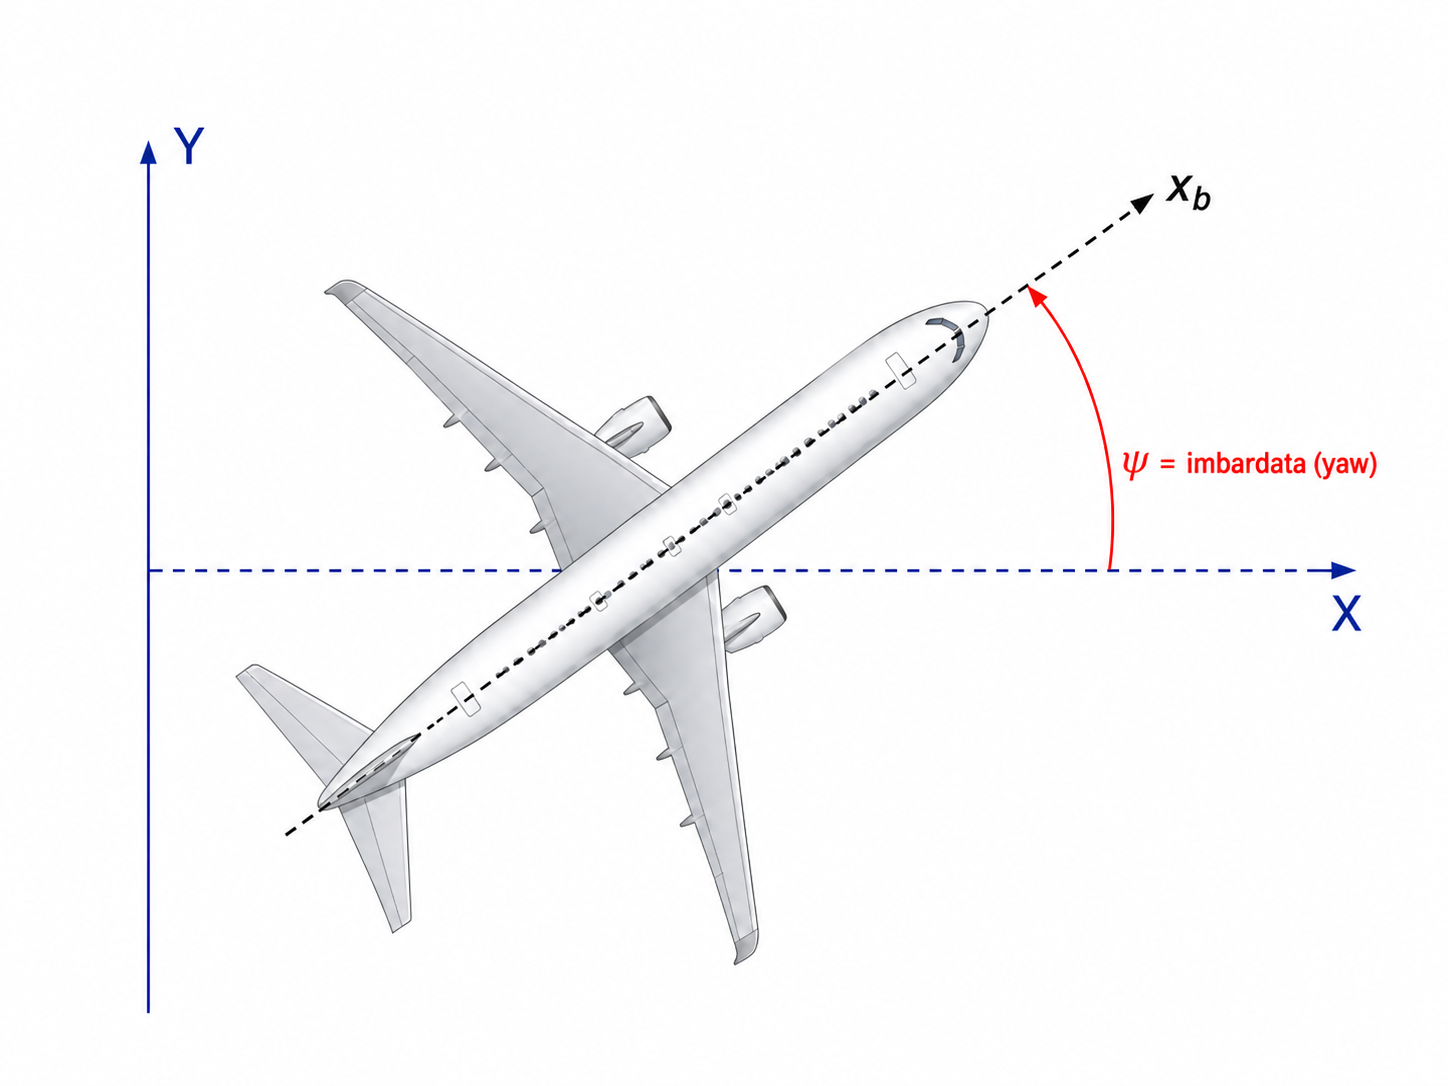
\includegraphics[width=\textwidth]{immagini/aereo1.PNG}
\end{minipage}
\hfill
\begin{minipage}{0.45\textwidth}
\centering
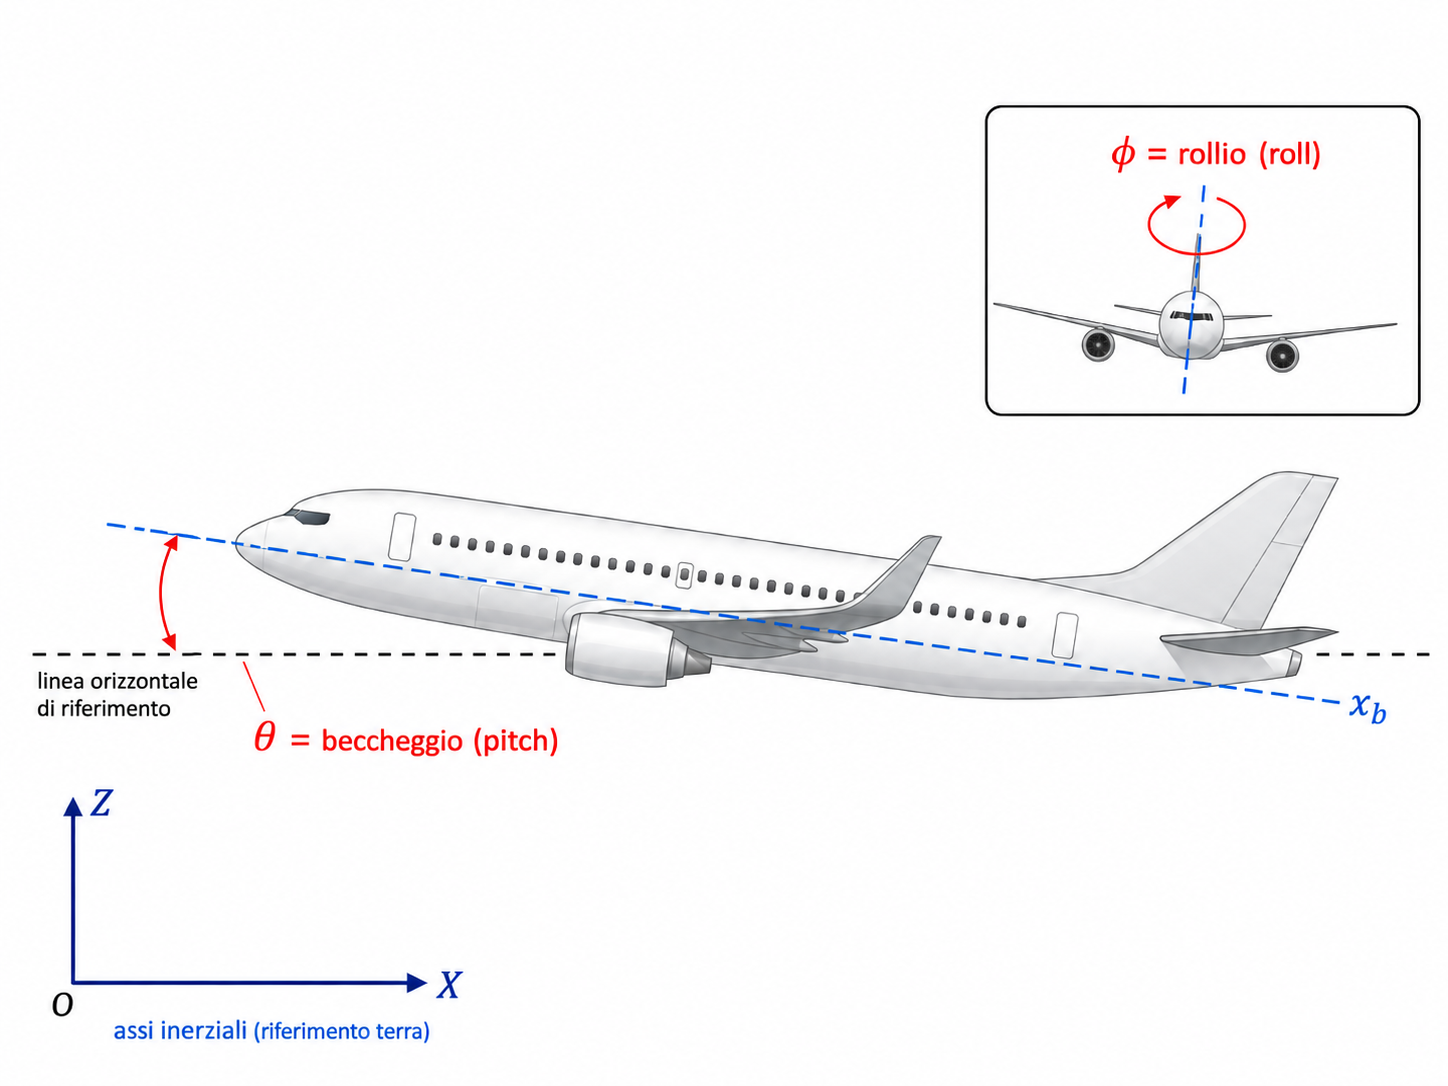
\includegraphics[width=\textwidth]{immagini/aereo2.PNG}
\end{minipage}
\end{center}

Presentiamo ora gli angoli di Eulero che, seppur più difficili da definire rispetto a quelli di Cardano, sono più utili ai nostri scopi.

\begin{definition}{}[Angoli di Eulero]
Consideriamo due riferimenti:
\[
\left\{O,\hat{\imath},\hat{\jmath},\hat{k}\right\}
\qquad \text{fisso}
\]
e
\[
\left\{O,\hat{\imath}',\hat{\jmath}',\hat{k}'\right\}
\qquad \text{mobile}.
\]

Definiamo gli angoli di Eulero come gli angoli associati alle  tre rotazioni antiorarie:

\begin{enumerate}[label=\roman*)]
\item Rotazione di un angolo $\varphi$ \textup{(precessione)} attorno all'asse $\hat{k}$ fino a quando $\hat{\imath}$ non interseca il piano definito da $\hat{\imath}'$, $\hat{\jmath}'$.

Chiamiamo $\hat{u}$ il versore dell'asse $\hat{\imath}$ trasportato dalla rotazione. $\hat{u}$ è detto versore della linea dei nodi.

\item Rotazione di un angolo $\theta$ \textup{(nutazione)} attorno alla linea dei nodi fino a che l'asse $\hat{k}$ va a sovrapporsi con $\hat{k}'$.

\item Rotazione di un angolo $\psi$ \textup{(rotazione propria)} attorno a $\hat{k}'$ fino a che $\hat{\imath}$, $\hat{\jmath}$ non si sovrappongono a $\hat{\imath}'$, $\hat{\jmath}'$.
\end{enumerate}
\end{definition}

\begin{center}
    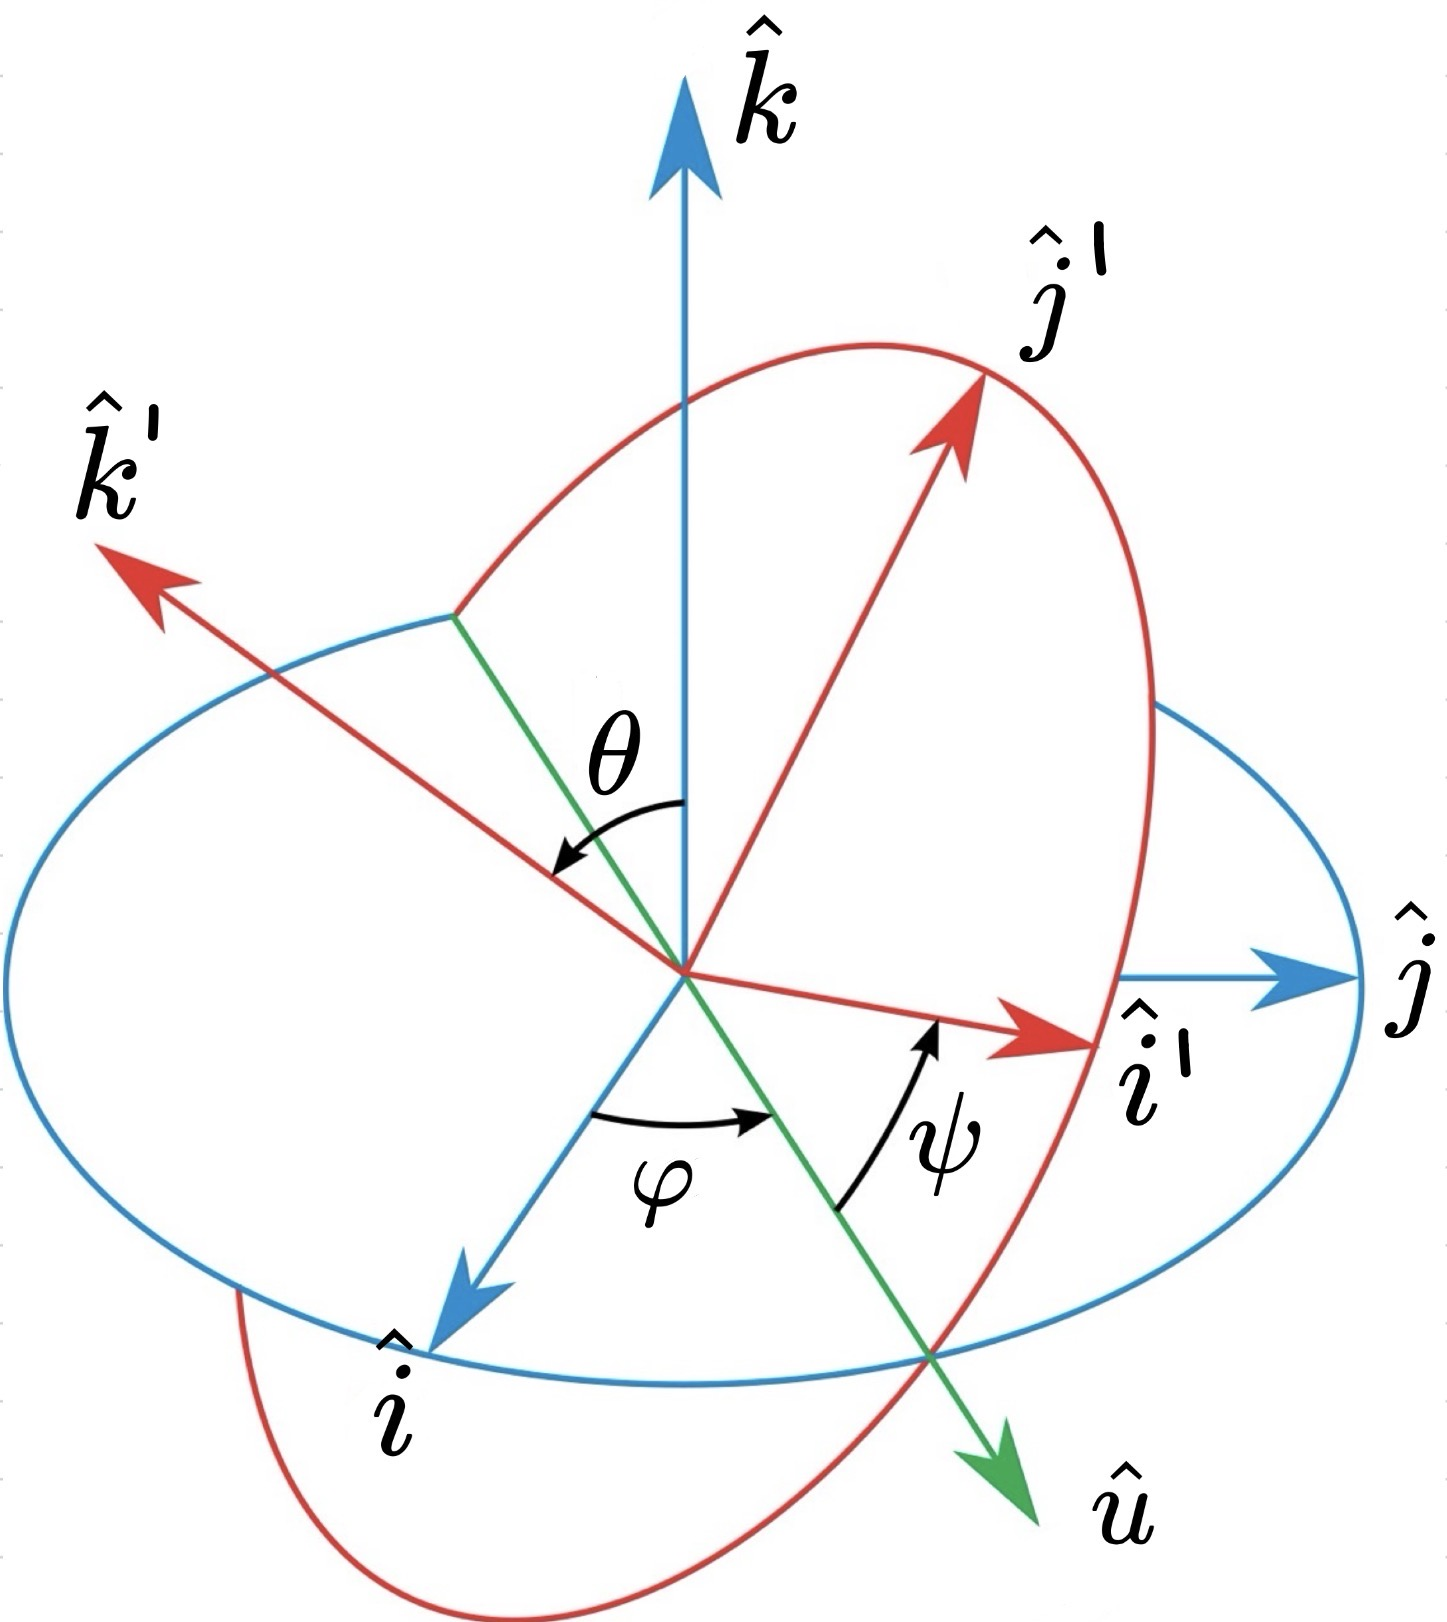
\includegraphics[scale=0.15]{immagini/angoli_eulero.jpg}
\end{center}

Per dare una trattazione matematica degli angoli di Eulero dobbiamo ricordare alcuni concetti di algebra lineare. Alcuni di questi sono già stati illustrati nel capitolo sulla formula fondamentale della cinematica e quindi li ricorderemo brevemente.

Consideriamo il gruppo delle rotazioni in $\mathbb{R}^n$
\[
R=\left\{R\in\mathbb{R}^{n,n}:\ R^TR=I_n,\ \det(R)=1\right\}.
\]

Questo è l'insieme di tutte le matrici ortogonali con determinante pari a $1$.

Iniziamo caratterizzando le rotazioni in $\mathbb{R}^2$. Consideriamo due basi ortonormali di $\mathbb{R}^2$
\[
\beta=\{\underline{e}_1,\underline{e}_2\},
\qquad
\beta'=\{\underline{e}_1',\underline{e}_2'\}
\]
tali che
\[
\underline{e}_1\cdot \underline{e}_1'=\underline{e}_2\cdot \underline{e}_2'=\cos\theta.
\]

\begin{center}
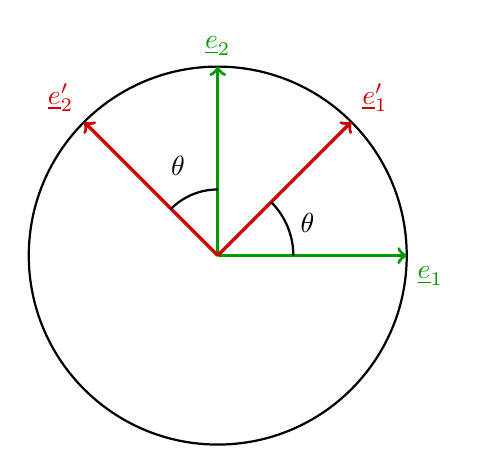
\begin{tikzpicture}[scale=1.2]
    % centro
    \coordinate (O) at (0,0);

    % cerchio
    \draw[thick] (O) circle (2);

    % assi / vettori della base beta
    \draw[->, very thick, green!60!black] (O) -- (2,0)
        node[below right] {$\underline{e}_1$};
    \draw[->, very thick, green!60!black] (O) -- (0,2)
        node[above] {$\underline{e}_2$};

    % vettori della base beta'
    \draw[->, very thick, red!80!black] (O) -- ({2*cos(45)},{2*sin(45)})
        node[above right] {$\underline{e}_1'$};
    \draw[->, very thick, red!80!black] (O) -- ({2*cos(135)},{2*sin(135)})
        node[above left] {$\underline{e}_2'$};

    % archi per theta
    \draw[thick] (0.8,0) arc[start angle=0,end angle=45,radius=0.8];
    \node at (0.95,0.35) {$\theta$};

    \draw[thick] ({0.7*cos(90)},{0.7*sin(90)}) arc[start angle=90,end angle=135,radius=0.7];
    \node at (-0.42,0.95) {$\theta$};
\end{tikzpicture}
\end{center}

Vogliamo trovare la rotazione $R \in \mathbb{R}^{2,2}$ tale che
\[
\underline{e}_1' = R\underline{e}_1,
\qquad
\underline{e}_2' = R\underline{e}_2.
\]

In particolare dovremmo trovare la matrice che rappresenta la rotazione rispetto a $\beta$ in partenza e in arrivo. Se però
\[
\underline{e}_1=(1,0)^T,
\qquad
\underline{e}_2=(0,1)^T,
\]
il conto è banale, infatti
\[
\underline{e}_1'=(\cos\theta,\sin\theta)^T,
\qquad
\underline{e}_2'=(-\sin\theta,\cos\theta)^T.
\]

Che implica che
\[
\begin{pmatrix}
r_{11} & r_{12}\\
r_{21} & r_{22}
\end{pmatrix}
\underline{e}_1
=
\begin{pmatrix}
r_{11} & r_{12}\\
r_{21} & r_{22}
\end{pmatrix}
\begin{pmatrix}
1\\
0
\end{pmatrix}
=
\begin{pmatrix}
r_{11}\\
r_{21}
\end{pmatrix}
=
\begin{pmatrix}
\cos\theta\\
\sin\theta
\end{pmatrix},
\]
\[
\begin{pmatrix}
r_{11} & r_{12}\\
r_{21} & r_{22}
\end{pmatrix}
\underline{e}_2
=
\begin{pmatrix}
r_{11} & r_{12}\\
r_{21} & r_{22}
\end{pmatrix}
\begin{pmatrix}
0\\
1
\end{pmatrix}
=
\begin{pmatrix}
r_{12}\\
r_{22}
\end{pmatrix}
=
\begin{pmatrix}
-\sin\theta\\
\cos\theta
\end{pmatrix}.
\]

Ovvero
\[
R=
\begin{pmatrix}
\cos\theta & -\sin\theta\\
\sin\theta & \cos\theta
\end{pmatrix}.
\]

È importante notare che $R$ è una rotazione attiva che mappa
\[
(\underline{e}_1,\underline{e}_2)
\quad \text{in} \quad
(\underline{e}_1',\underline{e}_2'),
\]
ovvero gira tutti i vettori del piano di un angolo $\theta$ in senso antiorario.

Per i nostri scopi però è più utile una matrice del cambio di base da $\beta$ a $\beta'$, ovvero una matrice che prende le componenti di un vettore $\underline{u}$ rispetto a $\beta$ e le mappa nelle componenti di $\underline{u}$ rispetto a $\beta'$.

Data l'importanza di $\beta$, le componenti di $\underline{u}$ rispetto a quest'ultima coincidono proprio con la descrizione che di solito diamo di $\underline{u}$, ovvero
\[
[\underline{u}]_{\beta}
=
\underline{u}
=
(u_1,u_2)^T.
\]

Ciò però non è più vero per quanto riguarda $\beta'$, ovvero
\[
\underline{u}
=
(u_1,u_2)^T
\neq
[\underline{u}]_{\beta'}
=
(u_1',u_2')^T.
\]

Ricordiamo infine che, in qualunque spazio vettoriale, la matrice $M_{\gamma}^{\gamma'}$ del cambio di base da $\gamma$ a $\gamma'$ è la matrice che rappresenta $\mathrm{id}_V$ rispetto a $\gamma$ in partenza e $\gamma'$ in arrivo.

Se lavoriamo con una base ortonormale, è particolarmente semplice ricavare le componenti di un vettore rispetto a quest'ultima. Infatti, se $\underline{u}\in \mathbb{R}^2$ e
\[
[\underline{u}]_{\beta}
=
(u_1,u_2)^T
=
\underline{u},
\qquad
[\underline{u}]_{\beta'}
=
(u_1',u_2')^T,
\]
è vero che
\[
(u_1',u_2')^T
=
\left(
\underline{u}\cdot \underline{e}_1',
\underline{u}\cdot \underline{e}_2'
\right)^T.
\]
Nel nostro caso
\[
(u_1',u_2')^T
=
\left(
\underline{u}\cdot \underline{e}_1',
\underline{u}\cdot \underline{e}_2'
\right)^T
=
\left(
(u_1\underline{e}_1+u_2\underline{e}_2)\cdot \underline{e}_1',
(u_1\underline{e}_1+u_2\underline{e}_2)\cdot \underline{e}_2'
\right)^T
\]
\[
=
\left(
u_1\,\underline{e}_1\cdot \underline{e}_1'
+
u_2\,\underline{e}_2\cdot \underline{e}_1',
u_1\,\underline{e}_1\cdot \underline{e}_2'
+
u_2\,\underline{e}_2\cdot \underline{e}_2'
\right)^T
\]
\[
=
\left(
u_1\cos\theta+u_2\sin\theta,
u_1\cos\left(\frac{\pi}{2}+\theta\right)+u_2\cos\theta
\right)^T
=
\left(
u_1\cos\theta+u_2\sin\theta,
-u_1\sin\theta+u_2\cos\theta
\right)^T
\]
\[
=
\begin{pmatrix}
\cos\theta & \sin\theta\\
-\sin\theta & \cos\theta
\end{pmatrix}
\begin{pmatrix}
u_1\\
u_2
\end{pmatrix}.
\]

Abbiamo quindi trovato che
\[
M_{\beta}^{\beta'}
=
R^T
=
R^{-1},
\]
ovvero è uguale alla rotazione attiva in senso orario di un angolo $\theta$.

Questo succede perché, quando operiamo un cambio di base, non stiamo effettivamente ruotando lo spazio, bensì stiamo cambiando il nostro punto di vista.

\begin{center}
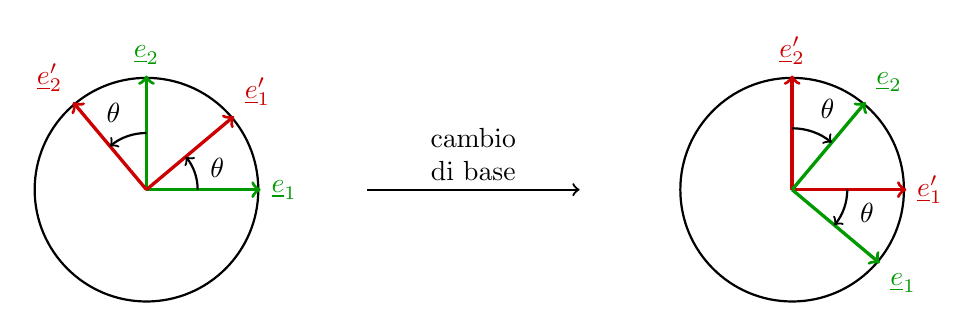
\begin{tikzpicture}[scale=1]

% grafico sinistro
\begin{scope}[shift={(0,0)}]
\draw[thick] (0,0) circle (1.42);

\draw[->, very thick, green!60!black] (0,0) -- (1.45,0)
node[right] {$\underline{e}_1$};
\draw[->, very thick, green!60!black] (0,0) -- (0,1.45)
node[above] {$\underline{e}_2$};

\draw[->, very thick, red!80!black] (0,0) -- ({1.45*cos(40)},{1.45*sin(40)})
node[above right] {$\underline{e}_1'$};
\draw[->, very thick, red!80!black] (0,0) -- ({1.45*cos(130)},{1.45*sin(130)})
node[above left] {$\underline{e}_2'$};

\draw[->, thick] (0.65,0) arc[start angle=0,end angle=40,radius=0.65];
\node at (0.9,0.28) {$\theta$};

\draw[->, thick] (0,0.72) arc[start angle=90,end angle=130,radius=0.72];
\node at (-0.42,0.98) {$\theta$};
\end{scope}

% freccia centrale
\draw[->, thick] (2.8,0) -- (5.5,0);
\node[align=center] at (4.15,0.45) {cambio\\di base};

% grafico destro
\begin{scope}[shift={(8.2,0)}]
\draw[thick] (0,0) circle (1.42);

\draw[->, very thick, red!80!black] (0,0) -- (1.45,0)
node[right] {$\underline{e}_1'$};
\draw[->, very thick, red!80!black] (0,0) -- (0,1.45)
node[above] {$\underline{e}_2'$};

\draw[->, very thick, green!60!black] (0,0) -- ({1.45*cos(-40)},{1.45*sin(-40)})
node[below right] {$\underline{e}_1$};
\draw[->, very thick, green!60!black] (0,0) -- ({1.45*cos(50)},{1.45*sin(50)})
node[above right] {$\underline{e}_2$};

\draw[->, thick] (0.7,0) arc[start angle=0,end angle=-40,radius=0.7];
\node at (0.95,-0.3) {$\theta$};

\draw[->, thick] (0,0.78) arc[start angle=90,end angle=50,radius=0.78];
\node at (0.45,1.02) {$\theta$};
\end{scope}

\end{tikzpicture}
\end{center}

I vettori ci appaiono così ruotati di un angolo $\theta$ in senso orario rispetto a come li vedevamo prima del cambio di base.

Un'altra classe di rotazioni che ci sono utili sono le rotazioni in $\mathbb{R}^3$ rispetto ad un asse fisso.

Partiremo con la descrizione della rotazione attiva attorno all'asse $z$, per poi descrivere il suo cambio di base associato. Daremo infine solo l'espressione delle rotazioni attive attorno all'asse $x$ e $y$ e dei loro cambi di base associati, in quanto questi si ricavano in modo analogo.

Sia
\[
\beta=\{\underline{e}_1,\underline{e}_2,\underline{e}_3\}
\]
la base canonica di $\mathbb{R}^3$ e sia
\[
\beta'=\{\underline{e}_1',\underline{e}_2',\underline{e}_3'\}
\]
la base ortonormale tale che
\[
\underline{e}_1\cdot \underline{e}_1'
=
\underline{e}_2\cdot \underline{e}_2'
=
\cos\theta,
\qquad
\underline{e}_3=\underline{e}_3'.
\]
\begin{center}
    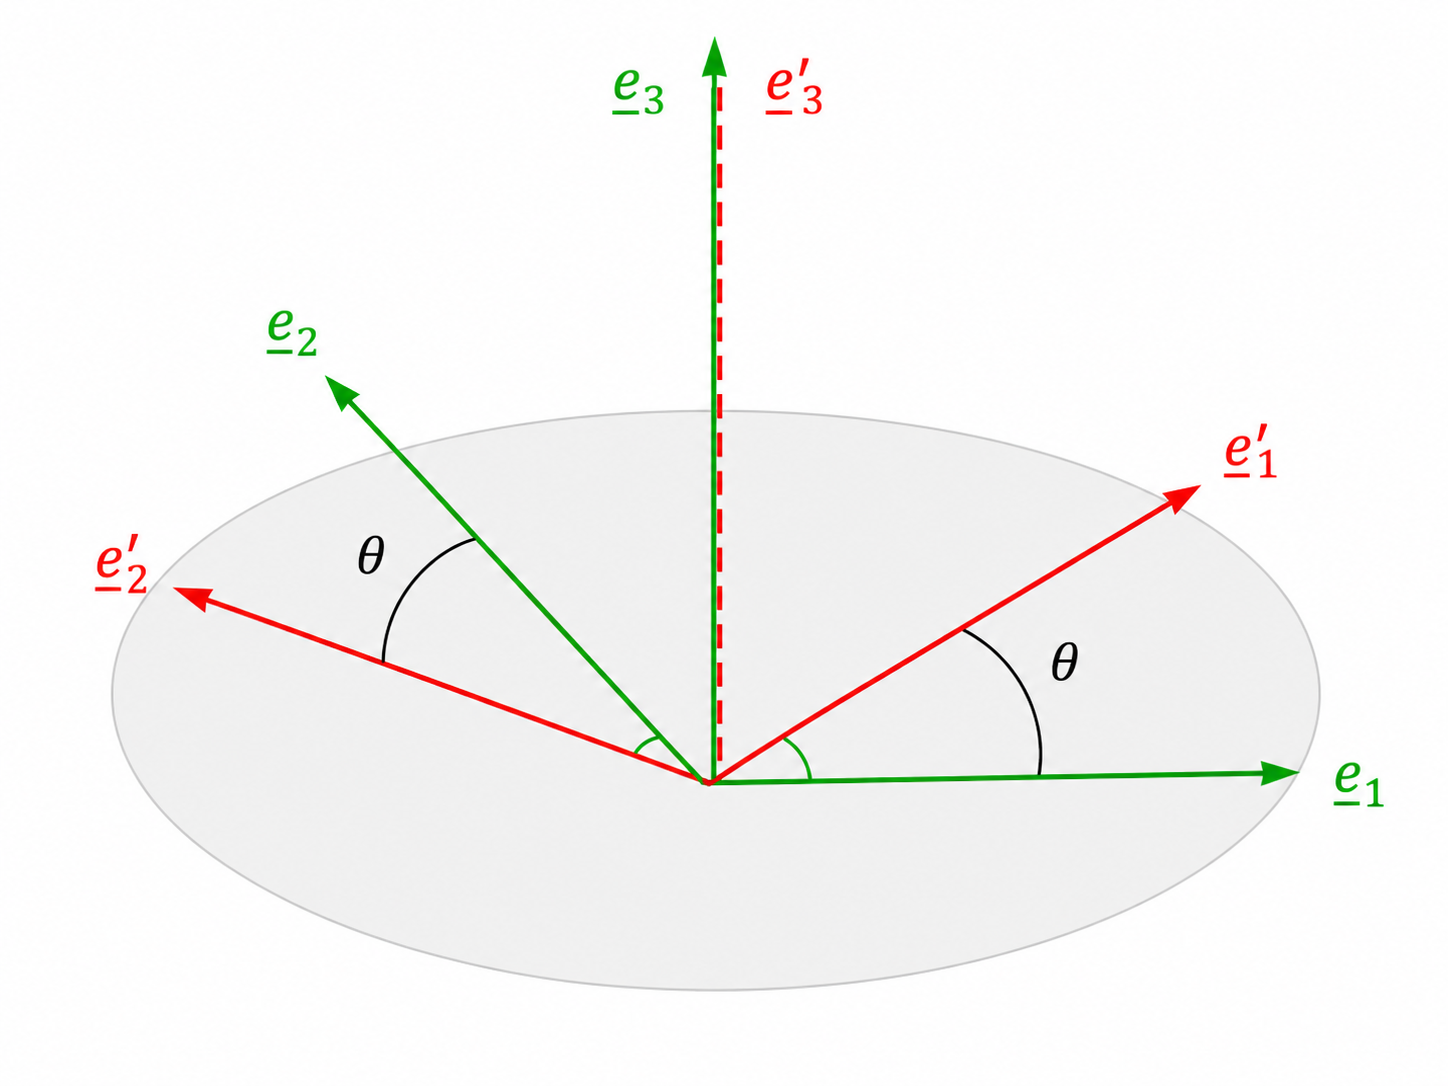
\includegraphics[scale=0.2]{immagini/basi_ortonormali.PNG}
\end{center}

Vogliamo trovare $R_z \in \mathbb{R}^{3,3}$ ortogonale tale che
\[
\underline{e}_1' = R_z \underline{e}_1,
\qquad
\underline{e}_2' = R_z \underline{e}_2,
\qquad
\underline{e}_3' = \underline{e}_3 = R_z\underline{e}_3.
\]

Procediamo come fatto nel caso bidimensionale:
\[
\underline{e}_1' = (\cos\theta,\sin\theta,0)^T,
\qquad
\underline{e}_2' = (-\sin\theta,\cos\theta,0)^T,
\qquad
\underline{e}_3' = (0,0,1)^T.
\]

\[
\begin{pmatrix}
r_{11} & r_{12} & r_{13}\\
r_{21} & r_{22} & r_{23}\\
r_{31} & r_{32} & r_{33}
\end{pmatrix}
\underline{e}_1
=
\begin{pmatrix}
r_{11} & r_{12} & r_{13}\\
r_{21} & r_{22} & r_{23}\\
r_{31} & r_{32} & r_{33}
\end{pmatrix}
\begin{pmatrix}
1\\
0\\
0
\end{pmatrix}
=
\begin{pmatrix}
r_{11}\\
r_{21}\\
r_{31}
\end{pmatrix}
=
\begin{pmatrix}
\cos\theta\\
\sin\theta\\
0
\end{pmatrix}
=
\underline{e}_1'.
\]

\[
\begin{pmatrix}
r_{11} & r_{12} & r_{13}\\
r_{21} & r_{22} & r_{23}\\
r_{31} & r_{32} & r_{33}
\end{pmatrix}
\underline{e}_2
=
\begin{pmatrix}
r_{11} & r_{12} & r_{13}\\
r_{21} & r_{22} & r_{23}\\
r_{31} & r_{32} & r_{33}
\end{pmatrix}
\begin{pmatrix}
0\\
1\\
0
\end{pmatrix}
=
\begin{pmatrix}
r_{12}\\
r_{22}\\
r_{32}
\end{pmatrix}
=
\begin{pmatrix}
-\sin\theta\\
\cos\theta\\
0
\end{pmatrix}
=
\underline{e}_2'.
\]

\[
\begin{pmatrix}
r_{11} & r_{12} & r_{13}\\
r_{21} & r_{22} & r_{23}\\
r_{31} & r_{32} & r_{33}
\end{pmatrix}
\underline{e}_3
=
\begin{pmatrix}
r_{11} & r_{12} & r_{13}\\
r_{21} & r_{22} & r_{23}\\
r_{31} & r_{32} & r_{33}
\end{pmatrix}
\begin{pmatrix}
0\\
0\\
1
\end{pmatrix}
=
\begin{pmatrix}
r_{13}\\
r_{23}\\
r_{33}
\end{pmatrix}
=
\begin{pmatrix}
0\\
0\\
1
\end{pmatrix}
=
\underline{e}_3'.
\]

Ovvero
\[
R_z
=
\begin{pmatrix}
\cos\theta & -\sin\theta & 0\\
\sin\theta & \cos\theta & 0\\
0 & 0 & 1
\end{pmatrix}.
\]

Anche in questo caso questa è la rotazione attiva. Siamo però più interessati al cambio di base da $\beta$ a $\beta'$, ovvero $M_{\beta}^{\beta'}$ tale che
\[
[\underline{u}]_{\beta'}
=
M_{\beta}^{\beta'}[\underline{u}]_{\beta}
\qquad
\forall \underline{u}\in\mathbb{R}^3.
\]

Come nel caso bidimensionale ci facciamo aiutare dal fatto che $\beta'$ è una base ortonormale e quindi, dato
\[
\underline{u}
=
[\underline{u}]_{\beta}
=
(u_1,u_2,u_3)^T
\in \mathbb{R}^3,
\]
è vero che
\[
[\underline{u}]_{\beta'}
=
\left(
\underline{u}\cdot \underline{e}_1',
\underline{u}\cdot \underline{e}_2',
\underline{u}\cdot \underline{e}_3'
\right)^T
\]
\[
=
\begin{pmatrix}
\left[u_1\underline{e}_1+u_2\underline{e}_2+u_3\underline{e}_3\right]\cdot \underline{e}_1'
\\[4pt]
\left[u_1\underline{e}_1+u_2\underline{e}_2+u_3\underline{e}_3\right]\cdot \underline{e}_2'
\\[4pt]
\left[u_1\underline{e}_1+u_2\underline{e}_2+u_3\underline{e}_3\right]\cdot \underline{e}_3'
\end{pmatrix}
\]
\[
=
\begin{pmatrix}
u_1\cos\theta+u_2\sin\theta
\\
-u_1\sin\theta+u_2\cos\theta
\\
u_3
\end{pmatrix}
=
\begin{pmatrix}
\cos\theta & \sin\theta & 0
\\
-\sin\theta & \cos\theta & 0
\\
0 & 0 & 1
\end{pmatrix}
\begin{pmatrix}
u_1\\
u_2\\
u_3
\end{pmatrix}.
\]

Anche qui abbiamo ottenuto che
\[
M_{\beta}^{\beta'}
=
R_z^T
=
R_z^{-1}.
\]

Il motivo è lo stesso del caso bidimensionale: non stiamo ruotando lo spazio, ma stiamo cambiando il nostro punto di vista.

Le matrici di rotazione rispetto all'asse $x$ e all'asse $y$ sono
\[
R_x
=
\begin{pmatrix}
1 & 0 & 0
\\
0 & \cos\theta & -\sin\theta
\\
0 & \sin\theta & \cos\theta
\end{pmatrix},
\qquad
R_y
=
\begin{pmatrix}
\cos\theta & 0 & \sin\theta
\\
0 & 1 & 0
\\
-\sin\theta & 0 & \cos\theta
\end{pmatrix}.
\]

I corrispondenti cambi di base sono
\[
R_x^T,
\qquad
R_y^T.
\]

Siamo finalmente pronti a dare una descrizione matematica agli angoli di Eulero. In particolare siano
\[
\gamma=\{\hat{\imath},\hat{\jmath},\hat{k}\},
\qquad
\gamma'=\{\hat{\imath}',\hat{\jmath}',\hat{k}'\},
\]
troviamo $M_{\gamma}^{\gamma'}$.

Le rotazioni che abbiamo descritto nella definizione degli angoli di Eulero sono le rotazioni attive date dalle matrici
\[
\text{(i)} \qquad
C^T=
\begin{pmatrix}
\cos\varphi & -\sin\varphi & 0\\
\sin\varphi & \cos\varphi & 0\\
0 & 0 & 1
\end{pmatrix},
\]
\[
\text{(ii)} \qquad
B^T=
\begin{pmatrix}
1 & 0 & 0\\
0 & \cos\theta & -\sin\theta\\
0 & \sin\theta & \cos\theta
\end{pmatrix},
\]
\[
\text{(iii)} \qquad
A^T=
\begin{pmatrix}
\cos\psi & -\sin\psi & 0\\
\sin\psi & \cos\psi & 0\\
0 & 0 & 1
\end{pmatrix}.
\]

Attenzione però al fatto che la nutazione e la rotazione propria non sono attorno agli assi $\hat{k}$ e $\hat{\imath}$ nel riferimento fisso, ma rispetto ad assi intermedi.

Scrivere che la rotazione attiva è data da
\[
A^TB^TC^T
\]
sarebbe quindi sbagliato. La giusta matrice è
\[
C^TB^TA^T.
\]
Vediamo perché.

\begin{enumerate}[label=\roman*)]
\item Il vettore $\hat{\imath}$ viene mandato in $\hat{u}$ attraverso $C^T$, ovvero
\[
\hat{u}=C^T\hat{\imath}.
\]

\item Ora dobbiamo applicare la rotazione $B^T$ attorno all'asse dei nodi. Per farlo facciamo un passo indietro: applichiamo la rotazione a $\hat{\imath}$, ovvero $B^T\hat{\imath}$, e poi riportiamo tutto attorno a $\hat{u}$, ovvero
\[
C^TB^T\hat{\imath}.
\]
In questo modo $\hat{\imath}$ viene ancora mappato in $\hat{u}$, infatti
\[
C^TB^T\hat{\imath}
=
C^T\hat{\imath}
=
\hat{u}.
\]

\item Infine vogliamo effettuare la rotazione attorno a $\hat{k}'$. Allo stesso modo torniamo indietro, applichiamo $A^T$ a $\hat{k}$, ovvero $A^T\hat{k}$, poi ruotiamo di nuovo con $C^TB^T$. Come verifica controlliamo dove viene mandato $\hat{k}$:
\[
C^TB^TA^T\hat{k}
=
C^TB^T\hat{k}
=
\hat{k}'.
\]
\end{enumerate}

Il cambio di base associato è quindi
\[
M_{\gamma}^{\gamma'}
=
(C^TB^TA^T)^T
=
ABC,
\]
con
\[
A=
\begin{pmatrix}
\cos\psi & \sin\psi & 0\\
-\sin\psi & \cos\psi & 0\\
0 & 0 & 1
\end{pmatrix},
\]
\[
B=
\begin{pmatrix}
1 & 0 & 0\\
0 & \cos\theta & \sin\theta\\
0 & -\sin\theta & \cos\theta
\end{pmatrix},
\]
\[
C=
\begin{pmatrix}
\cos\varphi & \sin\varphi & 0\\
-\sin\varphi & \cos\varphi & 0\\
0 & 0 & 1
\end{pmatrix}.
\]
\vspace{30pt}
\section{Il moto della trottola}

La trottola è un modello per un corpo rigido dotato di un asse di simmetria soggetto alla forza peso e con un punto fisso.

\begin{center}
    \begin{tikzpicture}[scale=1.15,>=Latex]

\coordinate (O) at (0,0);

% angoli dei vari assi
\def\angi{-145}
\def\angu{-112}
\def\angip{-55}
\def\angjp{42}
\def\angkp{125}

% assi fissi
\coordinate (I) at ($(O)+(\angi:4.2)$);
\coordinate (J) at ($(O)+(0:5.4)$);
\coordinate (K) at ($(O)+(90:4.8)$);

% assi principali d'inerzia
\coordinate (Ip) at ($(O)+(\angip:4.2)$);
\coordinate (Jp) at ($(O)+(\angjp:4.7)$);
\coordinate (Kp) at ($(O)+(\angkp:4.8)$);

% linea dei nodi
\coordinate (U) at ($(O)+(\angu:3.1)$);

% centro di massa su k'
\coordinate (G) at ($(O)+(\angkp:2.05)$);

%------------------------------------------------
% trottola stilizzata, allineata con k'
% disegnata inizialmente lungo l'asse y e poi ruotata
\begin{scope}[shift={(O)},rotate=35]

  % corpo principale
  \filldraw[fill=white,draw=black,thick]
    (0,0)
    .. controls (-0.10,0.26) and (-0.58,0.88) .. (-0.98,1.60)
    .. controls (-1.25,2.15) and (-1.22,2.88) .. (-0.58,3.35)
    .. controls (-0.36,3.52) and (-0.22,3.70) .. (-0.18,3.90)
    -- (0.18,3.90)
    .. controls (0.22,3.70) and (0.36,3.52) .. (0.58,3.35)
    .. controls (1.22,2.88) and (1.25,2.15) .. (0.98,1.60)
    .. controls (0.58,0.88) and (0.10,0.26) .. (0,0)
    -- cycle;

  % collarino vicino alla punta
  \draw[thick]
    (-0.16,0.52) .. controls (-0.08,0.60) and (0.08,0.60) .. (0.16,0.52);
  \draw[thick]
    (-0.13,0.44) .. controls (-0.05,0.50) and (0.05,0.50) .. (0.13,0.44);

  % anelli decorativi
  \draw[thick]
    (-0.76,1.78) .. controls (-0.32,1.98) and (0.32,1.98) .. (0.76,1.78);
  \draw[thick]
    (-0.94,2.42) .. controls (-0.40,2.66) and (0.40,2.66) .. (0.94,2.42);
  \draw[thick]
    (-0.74,3.02) .. controls (-0.28,3.22) and (0.28,3.22) .. (0.74,3.02);

  % pomello superiore
  \draw[thick]
    (-0.18,3.90) .. controls (-0.22,4.05) and (-0.30,4.15) .. (-0.18,4.25);
  \draw[thick]
    (0.18,3.90) .. controls (0.22,4.05) and (0.30,4.15) .. (0.18,4.25);
  \draw[thick] (0,4.25) ellipse[x radius=0.18,y radius=0.06];

\end{scope}
%------------------------------------------------
% assi fissi
\draw[->,very thick] (O) -- (J) node[right] {$\hat j$};
\draw[->,very thick] (O) -- (K) node[above] {$\hat k$};
\draw[->,very thick] (O) -- (I) node[below left] {$\hat i$};

% assi principali d'inerzia
\draw[->,red!80!black,dashed,thick] (O) -- (Kp) node[above left] {$\hat k'$};
\draw[->,red!80!black,dashed,thick] (O) -- (Jp) node[above right] {$\hat j'$};
\draw[->,red!80!black,dashed,thick] (O) -- (Ip) node[below right] {$\hat i'$};

% linea dei nodi
\draw[->,violet,very thick] (O) -- (U) node[below] {$\underline{u}$};



%------------------------------------------------
% centro di massa
\fill[green!60!black] (G) circle (2.4pt);
\node[above right=1pt,green!60!black] at (G) {$G$};

% forza peso
\draw[->,green!60!black,thick] (G) -- ++(0,-1.9) node[below left] {$m\underline{g}$};

% graffa per il segmento d = OG
\draw[
  green!60!black,
  thick,
  decorate,
  decoration={brace,amplitude=6pt}
]
  ($(O)+(215:0.30)$) -- ($(G)+(215:0.30)$)
  node[midway,left=8pt] {$d$};

%------------------------------------------------
% angoli di Eulero
\draw[orange!85!black,thick]
  ($(O)+(\angi:1.02)$)
  arc[start angle=\angi,end angle=\angu,radius=1.02];
\node[orange!85!black] at ($(O)+(-129:1.28)$) {$\varphi$};

\draw[orange!85!black,thick]
  ($(O)+(90:1.14)$)
  arc[start angle=90,end angle=\angkp,radius=1.14];
\node[orange!85!black] at ($(O)+(108:1.45)$) {$\theta$};

\draw[orange!85!black,thick]
  ($(O)+(\angu:0.84)$)
  arc[start angle=\angu,end angle=\angip,radius=0.84];
\node[orange!85!black] at ($(O)+(-84:1.02)$) {$\psi$};

% origine
\fill (O) circle (2pt);

\end{tikzpicture}
\end{center}

Impostiamo due sistemi di riferimento:
\[
\beta=\{\hat{i},\hat{j},\hat{k}\}
\quad \text{fisso}
\qquad \text{e} \qquad
\beta'=\{\hat{i}',\hat{j}',\hat{k}'\}
\quad \text{solidale}.
\]

L'asse \(\hat{k}'\) è anche asse di simmetria.

Scriviamo le equazioni del moto. Il sistema ha \(3\) gradi di libertà.
Scegliamo come coordinate libere gli angoli di Eulero.

Il sistema ha energia potenziale
\[
V = mgd\cos\theta.
\]

Se impostiamo \(\hat{i}',\hat{j}',\hat{k}'\) lungo gli assi principali d'inerzia, il tensore d'inerzia risulta diagonale:
\[
I_C =
\begin{pmatrix}
I & 0 & 0\\
0 & I & 0\\
0 & 0 & I_0
\end{pmatrix}.
\]

\[
T =
\frac{1}{2}
[\underline{\omega}]_{\beta'} \cdot I_C [\underline{\omega}]_{\beta'}
\]
dove \([\underline{\omega}]_{\beta'}\) è il vettore delle componenti di
\(\underline{\omega}\) rispetto a \(\beta'\).

Scegliamo, per ragioni fisiche, di rappresentare
\[
\underline{\omega}
=
\dot{\varphi}\hat{k}
+
\dot{\theta}\,\underline{u}
+
\dot{\psi}\hat{k}'.
\]

Dobbiamo scrivere \(\underline{\omega}\) lungo
\[
\{\hat{i}',\hat{j}',\hat{k}'\}.
\]

Usiamo i \(3\) cambi di base ABC definiti nel paragrafo precedente:
\[
\begin{pmatrix}
\cos\psi & \sin\psi & 0\\
-\sin\psi & \cos\psi & 0\\
0 & 0 & 1
\end{pmatrix}
\begin{pmatrix}
\dot{\theta}\\
0\\
0
\end{pmatrix}
=
\dot{\theta}
\begin{pmatrix}
\cos\psi\\
-\sin\psi\\
0
\end{pmatrix}.
\]

Quindi
\[
\dot{\theta}\,\underline{u}
=
\dot{\theta}\cos\psi\,\hat{i}'
-
\dot{\theta}\sin\psi\,\hat{j}'.
\]
\[
\begin{pmatrix}
\cos\psi & \sin\psi & 0\\
-\sin\psi & \cos\psi & 0\\
0 & 0 & 1
\end{pmatrix}
\begin{pmatrix}
1 & 0 & 0\\
0 & \cos\theta & \sin\theta\\
0 & -\sin\theta & \cos\theta
\end{pmatrix}
\begin{pmatrix}
0\\
0\\
\dot{\varphi}
\end{pmatrix}
=
\begin{pmatrix}
\cos\psi & \sin\psi & 0\\
-\sin\psi & \cos\psi & 0\\
0 & 0 & 1
\end{pmatrix}
\begin{pmatrix}
0\\
\sin\theta\,\dot{\varphi}\\
\cos\theta\,\dot{\varphi}
\end{pmatrix}
=
\]

\[
=
\begin{pmatrix}
\sin\psi\sin\theta\,\dot{\varphi}\\
\cos\psi\sin\theta\,\dot{\varphi}\\
\cos\theta\,\dot{\varphi}
\end{pmatrix}^{T}
\]

\[
\Rightarrow
\dot{\varphi}\hat{k}
=
\sin\psi\sin\theta\,\dot{\varphi}\,\hat{i}'
+
\cos\psi\sin\theta\,\dot{\varphi}\,\hat{j}'
+
\cos\theta\,\dot{\varphi}\,\hat{k}'.
\]

\[
\Rightarrow
\underline{\omega}
=
\left(
\dot{\theta}\cos\psi
+
\sin\psi\sin\theta\,\dot{\varphi}
\right)\hat{i}'
+
\left(
-\dot{\theta}\sin\psi
+
\cos\psi\sin\theta\,\dot{\varphi}
\right)\hat{j}'
+
\left(
\dot{\psi}
+
\cos\theta\,\dot{\varphi}
\right)\hat{k}'.
\]

Possiamo quindi scrivere l'energia cinetica.

\[
\begin{aligned}
2T
&=
[\underline{\omega}]_{\beta'}\cdot I_C[\underline{\omega}]_{\beta'}\\
&=
I\left(
\dot{\theta}\cos\psi
+
\sin\psi\sin\theta\,\dot{\varphi}
\right)^2
+
I\left(
-\dot{\theta}\sin\psi
+
\dot{\varphi}\cos\psi\sin\theta
\right)^2
+
I_0
\left(
\dot{\psi}
+
\dot{\varphi}\cos\theta
\right)^2.
\end{aligned}
\]

\[
\begin{aligned}
&=
I\left(
\dot{\theta}^2\cos^2\psi
+
\sin^2\psi\sin^2\theta\,\dot{\varphi}^2
+
2\dot{\theta}\cos\psi\sin\psi\sin\theta\,\dot{\varphi}
\right)\\
&\quad+
I\left(
\dot{\theta}^2\sin^2\psi
+
\dot{\varphi}^2\cos^2\psi\sin^2\theta
-
2\dot{\theta}\sin\psi\cos\psi\sin\theta\,\dot{\varphi}
\right)\\
&\quad+
I_0
\left(
\dot{\psi}
+
\dot{\varphi}\cos\theta
\right)^2\\
&=
I\left(
\dot{\theta}^2\cos^2\psi
+
\sin^2\psi\sin^2\theta\,\dot{\varphi}^2
+
\dot{\theta}^2\sin^2\psi
+
\dot{\varphi}^2\cos^2\psi\sin^2\theta
\right)\\
&\quad+
I_0
\left(
\dot{\psi}
+
\dot{\varphi}\cos\theta
\right)^2\\
&=
I\dot{\theta}^2
+
I\sin^2\theta\,\dot{\varphi}^2
+
I_0
\left(
\dot{\psi}
+
\dot{\varphi}\cos\theta
\right)^2.
\end{aligned}
\]

\[
\mathcal{L}
=
T-V
=
\frac{I}{2}
\left(
\dot{\theta}^2
+
\sin^2\theta\,\dot{\varphi}^2
\right)
+
\frac{I_0}{2}
\left(
\dot{\psi}
+
\dot{\varphi}\cos\theta
\right)^2
-
mgd\cos\theta.
\]

Notiamo che \(\mathcal{L}\) non dipende da \(\varphi\) e da \(\psi\), allora
\[
\frac{\partial \mathcal{L}}{\partial \dot{\varphi}},
\qquad
\frac{\partial \mathcal{L}}{\partial \dot{\psi}}
\]
sono costanti nel tempo.

\[
\frac{\partial \mathcal{L}}{\partial \dot{\varphi}}
=
I\sin^2\theta\,\dot{\varphi}
+
I_0
\left(
\dot{\psi}
+
\dot{\varphi}\cos\theta
\right)\cos\theta
=
\left.
\frac{\partial \mathcal{L}}{\partial \dot{\varphi}}
\right|_{t=0}
=
Ib,
\qquad b\in\mathbb{R}.
\]

\[
\frac{\partial \mathcal{L}}{\partial \dot{\psi}}
=
I_0
\left(
\dot{\psi}
+
\dot{\varphi}\cos\theta
\right)
=
\left.
\frac{\partial \mathcal{L}}{\partial \dot{\psi}}
\right|_{t=0}
=
Ia,
\qquad a\in\mathbb{R}.
\]

Vogliamo ottenere \(2\) equazioni disaccoppiate. Sostituisco \(Ia\) nella prima

\[
I\sin^2\theta\,\dot{\varphi}
+
Ia\cos\theta
=
Ib
\Rightarrow
\sin^2\theta\,\dot{\varphi}
+
a\cos\theta
=
b
\Rightarrow
\dot{\varphi}
=
\frac{b-a\cos\theta}{\sin^2\theta}.
\]

La trottola è sottoposta solo a forze conservative e quindi l'energia meccanica si conserva

\[
\frac{I}{2}
\left(
\dot{\theta}^2
+
\sin^2\theta\,\dot{\varphi}^2
\right)
+
\frac{I_0}{2}
\left(
\dot{\psi}
+
\dot{\varphi}\cos\theta
\right)^2
+
mgd\cos\theta
=
E.
\]
Da
\[
\frac{\partial \mathcal{L}}{\partial \dot{\psi}} = Ia
\]
otteniamo
\[
\left(\dot{\psi}+\dot{\varphi}\cos\theta\right)^2
=
\frac{I^2a^2}{I_0^2}
\]
e quindi
\[
\frac{I}{2}
\left(
\dot{\theta}^2+\sin^2\theta\,\dot{\varphi}^2
\right)
+
\frac{I^2a^2}{2I_0}
+
mgd\cos\theta
=
E.
\]

Dal momento che
\[
\dot{\varphi}
=
\frac{b-a\cos\theta}{\sin^2\theta},
\]
si ha
\[
\frac{I}{2}
\left(
\dot{\theta}^2
+
\frac{\left(b-a\cos\theta\right)^2}{\sin^2\theta}
\right)
+
\frac{I^2a^2}{2I_0}
+
mgd\cos\theta
=
E.
\]

\[
\Rightarrow
\frac{2E}{I}
=
\frac{2}{I}\cdot\frac{I^2a^2}{2I_0}
+
\dot{\theta}^2
+
\frac{\left(b-a\cos\theta\right)^2}{\sin^2\theta}
+
\frac{2}{I}mgd\cos\theta.
\]

\[
\Rightarrow
\dot{\theta}^2
+
\frac{\left(b-a\cos\theta\right)^2}{\sin^2\theta}
+
\frac{2}{I}mgd\cos\theta
=
\frac{2E}{I}
-
\frac{Ia^2}{I_0}.
\]

Ponendo
\[
\alpha
=
\frac{2E}{I}
-
\frac{Ia^2}{I_0}
\qquad
\text{e}
\qquad
\beta
=
\frac{2}{I}mgd,
\]
ottengo
\[
\dot{\theta}^2
+
\frac{\left(b-a\cos\theta\right)^2}{\sin^2\theta}
+
\beta\cos\theta
=
\alpha
\Rightarrow
\dot{\theta}^2
=
\alpha
-
\frac{\left(b-a\cos\theta\right)^2}{\sin^2\theta}
-
\beta\cos\theta.
\]

Abbiamo ottenuto un'equazione differenziale del primo ordine disaccoppiata.

Proviamo un cambio di variabile

\[
\Rightarrow
\dot{\theta}^2
=
\alpha
-
\frac{\left(b-a\cos\theta\right)^2}{1-\cos^2\theta}
-
\beta\cos\theta.
\]

\[
\Rightarrow
\left(1-\cos^2\theta\right)\dot{\theta}^2
=
\alpha\left(1-\cos^2\theta\right)
-
\left(b-a\cos\theta\right)^2
-
\beta\left(1-\cos^2\theta\right)\cos\theta.
\]

Pongo
\[
u=\cos\theta,
\qquad
\dot{u}=-\sin\theta\,\dot{\theta},
\qquad
\dot{u}^2
=
\sin^2\theta\,\dot{\theta}^2
=
\left(1-\cos^2\theta\right)\dot{\theta}^2.
\]

\[
\dot{u}^2
=
\alpha\left(1-u^2\right)
-
\left(b-au\right)^2
-
\beta\left(1-u^2\right)u.
\]

\[
\Rightarrow
\dot{u}^2
=
(\alpha-\beta u)(1-u^2)-(b-au)^2
\qquad
\alpha,\beta,a,b \text{ noti}
\]

Studiamo segni e zeri del polinomio \(p(u)\) a secondo membro. Iniziamo con i limiti agli estremi del dominio

\[
\lim_{u\to +\infty} (\alpha-\beta u)(1-u^2)-(b-au)^2
=
\lim_{u\to +\infty} \beta u^3
=
+\infty
\]

\[
\lim_{u\to -\infty} (\alpha-\beta u)(1-u^2)-(b-au)^2
=
\lim_{u\to -\infty} \beta u^3
=
-\infty
\]

Ricordando che
\[
\beta=\frac{2}{I}mgd>0
\]

Notiamo ora che \(p(1)=p(-1)=-(b-a)^2<0\). L'equazione differenziale di incognita \(u(t)\) è una EDO del primo ordine per la quale siamo certi esista una soluzione locale (teorema di esistenza ed unicità). La soluzione può esistere solo se \(p(u)\) ammette valori positivi nell'intervallo in \(S\subseteq[-1,1]\). Infatti essendo \(\dot{u}^2=p(u)\) allora \(p(u)\) deve essere non negativo ed inoltre \(u=\cos\theta \Rightarrow u\in[-1,1]\). Possiamo anche escludere l'ipotesi \(\dot{u}^2=0\ \forall t\) perché osserviamo un moto e quindi in almeno un istante \(t_0\) deve essere stato \((\dot{u}(t_0))^2>0\). Allora esiste \(u_0\in[-1,1]\) tale che \(p(u_0)>0\). Sappiamo quindi che

\[
\lim_{u\to -\infty} p(u)=-\infty
\qquad
p(-1)<0
\qquad
p(u_0)>0
\qquad
p(1)<0
\qquad
\lim_{u\to +\infty} p(u)=+\infty
\]

Per il teorema di esistenza degli zeri (\(\mathbb{R}\) connesso, \(p(u)\) continua) esistono \(u_1,u_2,u_3\) tali che

\[
p(u_1)=p(u_2)=p(u_3)=0
\qquad
-1<u_1<u_0
\qquad
u_0<u_2<1
\qquad
1<u_3
\]

\begin{center}
\begin{tikzpicture}[scale=1.15,>=Latex]
  % assi
  \draw[->] (-1.4,0) -- (2.4,0);
  \draw[->] (0,-1.8) -- (0,2.0);

  % tacche e etichette
  \draw (-1,0.08) -- (-1,-0.08);
  \node[above] at (-1,0) {$-1$};

  \draw (1,0.08) -- (1,-0.08);
  \node[above] at (1,0) {$1$};

  % curva
  \draw[thick]
    plot[smooth] coordinates {
      (-0.20,-1.55)
      (0.20,0)
      (0.48,0.72)
      (0.70,0)
      (1.05,-0.72)
      (1.60,0)
      (2.08,1.55)
    };

  % punti/etichette degli zeri
  \fill (0.20,0) circle (1.4pt);
  \fill (0.70,0) circle (1.4pt);
  \fill (1.60,0) circle (1.4pt);

  \node[below] at (0.20,0) {$u_1$};
  \node[below] at (0.70,0) {$u_2$};
  \node[below] at (1.60,0) {$u_3$};
\end{tikzpicture}
\end{center}

Concludiamo quindi che il moto ammesso si ha per \(u_1\leq u\leq u_2\)

\[
\Rightarrow
\cos\theta_1\leq\cos\theta\leq\cos\theta_2
\Rightarrow
\theta_2\leq\theta\leq\theta_1
\]

ovvero l'asse \(\hat{k}'\) deve muoversi in una corona circolare fissata.

Un'ulteriore condizione sul moto può essere ricavata dal segno di \(\dot{\varphi}\).

\begin{itemize}
  \item Se \(\dot{\varphi}>0\) la traiettoria dell'asse \(\hat{k}'\) è semplice.
  \item Se \(\dot{\varphi}\) assume sia valori positivi che negativi la traiettoria dell'asse \(\hat{k}'\) presenta autointersezioni, infatti se cambia segno l'asse torna indietro.
\end{itemize}

\[
\dot{\varphi}=\frac{b-a\cos\theta}{\sin^2\theta}\geq 0
\iff
b-a\cos\theta\geq 0
\iff
\cos\theta\leq \frac{b}{a}
\]

\begin{center}
\begin{tikzpicture}[scale=1.18,>=Latex]

%========================================
% figura sinistra
%========================================
\begin{scope}[shift={(-4.9,0)}]

  \def\R{1.9}
  \pgfmathsetmacro{\yu}{0.78}
  \pgfmathsetmacro{\yl}{0.12}
  \pgfmathsetmacro{\xu}{sqrt(\R*\R-\yu*\yu)}
  \pgfmathsetmacro{\xl}{sqrt(\R*\R-\yl*\yl)}

  % assi
  \draw[->,thick] (0,0) -- (0,2.55);
  \draw[->,thick] (0,0) -- (4.05,0);
  \draw[->,thick] (0,0) -- (-2.55,-2.75);

  % sfera
  \draw[thick] (0,0) circle (\R);

  \begin{scope}
    \clip (0,0) circle (\R);

    % parallelo superiore: estremi sul bordo della sfera
    \draw[orange!85!black,thick]
      (-\xu,\yu)
      .. controls (-0.95,0.50) and (0.95,0.50) ..
      (\xu,\yu);

    % parallelo inferiore: estremi sul bordo della sfera
    \draw[orange!85!black,thick]
      (-\xl,\yl)
      .. controls (-0.95,-0.18) and (0.95,-0.18) ..
      (\xl,\yl);

    % traiettoria semplice, interamente compresa tra i due paralleli
    \draw[red,thick,samples=140,domain=-1.45:1.45,smooth,variable=\x]
      plot
      (
        \x,
        {0.35 + 0.21*sin(140*\x) - 0.06*\x*\x}
      );
  \end{scope}

  \node[orange!85!black] at (-0.62,0.86) {$\theta_2$};
  \node[orange!85!black] at (-1.08,-0.43) {$\theta_1$};

\end{scope}

%========================================
% figura destra
%========================================
\begin{scope}[shift={(4.9,0)}]

  \def\R{1.9}
  \pgfmathsetmacro{\yu}{0.78}
  \pgfmathsetmacro{\yl}{0.12}
  \pgfmathsetmacro{\xu}{sqrt(\R*\R-\yu*\yu)}
  \pgfmathsetmacro{\xl}{sqrt(\R*\R-\yl*\yl)}

  % assi
  \draw[->,thick] (0,0) -- (0,2.55);
  \draw[->,thick] (0,0) -- (4.05,0);
  \draw[->,thick] (0,0) -- (-2.55,-2.75);

  % sfera
  \draw[thick] (0,0) circle (\R);

  \begin{scope}
    \clip (0,0) circle (\R);

    % parallelo superiore: estremi sul bordo della sfera
    \draw[orange!85!black,thick]
      (-\xu,\yu)
      .. controls (-0.95,0.50) and (0.95,0.50) ..
      (\xu,\yu);

    % parallelo inferiore: estremi sul bordo della sfera
    \draw[orange!85!black,thick]
      (-\xl,\yl)
      .. controls (-0.95,-0.18) and (0.95,-0.18) ..
      (\xl,\yl);

    % traiettoria con autointersezioni, sempre dentro la corona
    \draw[red,thick,samples=260,domain=0:1,smooth,variable=\t]
      plot
      (
        {-1.45 + 2.90*\t + 0.32*sin(1080*\t)},
        {0.34 + 0.15*cos(1080*\t)}
      );
  \end{scope}

  \node[orange!85!black] at (-0.62,0.86) {$\theta_2$};
  \node[orange!85!black] at (-1.08,-0.43) {$\theta_1$};

\end{scope}

\end{tikzpicture}
\end{center}

\begin{oss}{}
Il momento delle forze esterne con polo \(O\) è
\[
\underline{M}=d\,\hat{k}'\wedge -mg\,\hat{k}
\]
che è sempre perpendicolare al piano \(\mathrm{span}\{\hat{k}',\hat{k}\}\).

Il momento angolare ha componenti lungo \(\hat{k}\) e lungo \(\hat{k}'\) che si conservano. Si può dimostrare che questo corrisponde all'integrale primo del moto
\[
\frac{\partial \mathcal{L}}{\partial \dot{\varphi}}=\mathrm{cost.}
\]
\end{oss}



\begin{example}{}
Studiamo il moto del sistema in figura.

\begin{figure}
    \centering
    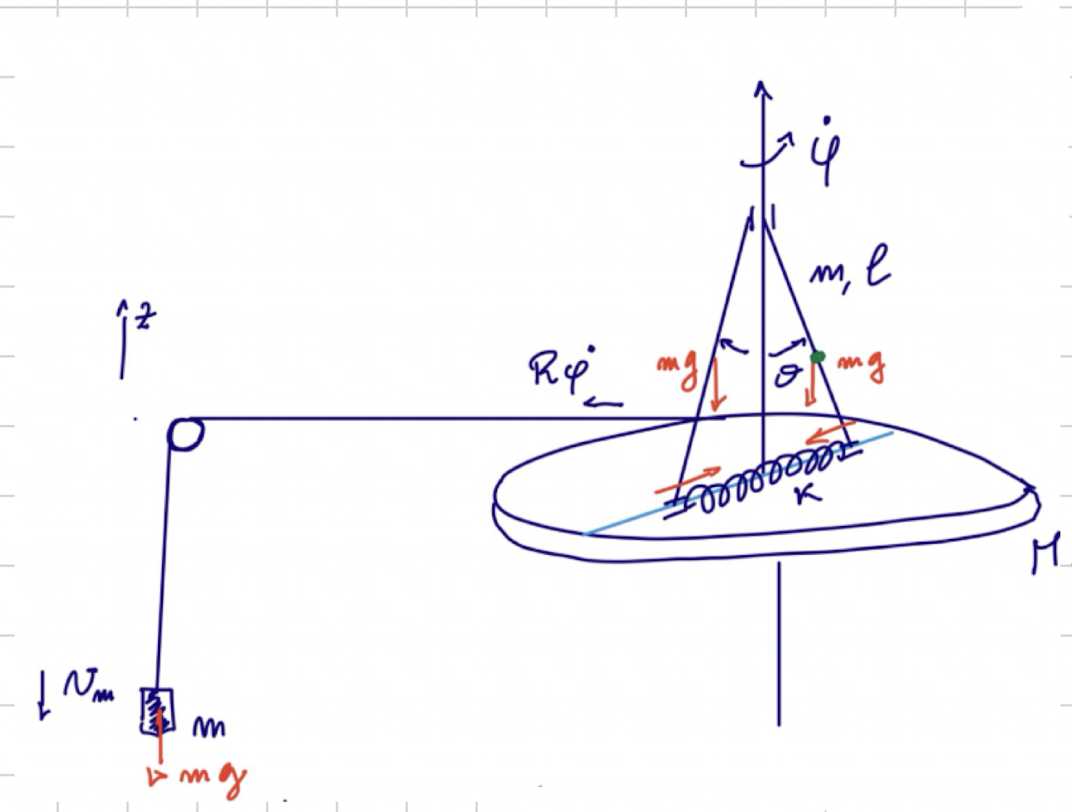
\includegraphics[width=0.55\textwidth]{immagini/piattaforma_rotante}
\end{figure}

Il disco ha massa \(M\) e raggio \(R\), le aste hanno entrambe massa \(m\) e lunghezza \(\ell\), il peso ha massa \(m\), il filo rotola senza strisciare attorno al disco. Il disco ruota attorno ad un asse principale d'inerzia e quindi ruota in un piano fisso. La molla ha costante elastica \(k\).

Il sistema ha due gradi di libertà. Scegliamo come coordinate libere \(\varphi\), angolo di rotazione del disco, e \(\theta\), angolo in figura.

La velocità del filo è uniforme ed uguale a \(R\dot{\varphi}\) (puro rotolamento). Allora
\[
y_m=-R\varphi
\]
supponendo che \(y_m(0)=0\).

Scriviamo l'energia potenziale del sistema.

\[
V=V^m+2V^{\text{peso asta}}+V^{\text{molla}}
\]

\[
V^m=mgy_m=-mgR\varphi
\]

\[
V^{\text{peso asta}}
=
mg\frac{\ell}{2}\cos\theta
\]

\[
V^{\text{molla}}
=
\frac{k}{2}\left(2\ell\sin\theta\right)^2
=
\frac{k}{2}4\ell^2\sin^2\theta
=
2k\ell^2\sin^2\theta
\]

\[
V
=
-mgR\varphi
+
2mg\frac{\ell}{2}\cos\theta
+
2k\ell^2\sin^2\theta
=
-mgR\varphi
+
mg\ell\cos\theta
+
2k\ell^2\sin^2\theta
\]

Calcoliamo ora l'energia cinetica

\[
T=T^{\text{disco}}+2T^{\text{asta}}+T^m
\]

\[
T^{\text{disco}}
=
\frac{MR^2}{2}\frac{\dot{\varphi}^2}{2}
\]

\[
T^m
=
\frac{m}{2}\dot{y}_m^2
=
\frac{m}{2}R^2\dot{\varphi}^2
\]

\[
T^{\text{asta}}
=
\frac{mv_G^2}{2}
+
\frac{\underline{\omega}_G I_G \underline{\omega}_G}{2}
\]

\(I_G\), \(\underline{\omega}\) rappresentati nelle componenti principali d'inerzia.
Partiamo dalla velocità del centro di massa.
\begin{center}
\begin{tikzpicture}[scale=1.2,>=Latex]

% punti principali
\coordinate (O) at (0,0);
\coordinate (P) at (0,2.9);
\coordinate (L) at (-1.2,0.75);
\coordinate (R) at (1.05,0.75);
\coordinate (G) at (-0.58,1.86);

% asse verticale
\draw[thick,->] (0,-1.4) -- (0,3.65) node[above] {$\hat z$};

% freccia che gira attorno all'asse verticale
\draw[thick,->]
  (0.38,3.15)
  arc[start angle=20,end angle=320,x radius=0.38,y radius=0.16];
\node[right] at (0.42,3.18) {$\dot{\varphi}$};

% aste
\draw[thick] (P) -- (L);
\draw[thick] (P) -- (R);

% centro di massa
\fill (G) circle (1.8pt);
\node[left] at (G) {$G$};

% graffa per l/2
\draw[
  thick,
  decorate,
  decoration={brace,amplitude=5pt}
]
  ($(G)+(-0.08,0.03)$) -- ($(P)+(-0.08,0.03)$)
  node[midway,left=3pt] {$\dfrac{\ell}{2}$};

% angolo theta
\draw[thick]
  ($(P)+(270:0.48)$)
  arc[start angle=270,end angle=300,radius=0.48];
\node[right] at ($(P)+(266:0.68)$) {$\theta$};

% terna locale rossa
\coordinate (A) at (0.55,1.82);

% asse k
\draw[->,red,thick] (A) -- ++(0,0.72) node[above] {$\hat{k}$};

% asse n
\draw[->,red,thick] (A) -- ++(0.95,0) node[right] {$\hat{n}$};

% asse t entrante: cerchietto con x
\draw[red,thick] (A) circle (0.12);
\draw[red,thick] ($(A)+(-0.07,-0.07)$) -- ($(A)+(0.07,0.07)$);
\draw[red,thick] ($(A)+(-0.07,0.07)$) -- ($(A)+(0.07,-0.07)$);
\node[red,below left] at ($(A)+(-0.02,-0.02)$) {$\hat{t}$};

\end{tikzpicture}
\end{center}

\[
\underline{v}_G
=
\left(
\frac{\ell}{2}\sin\theta\,\dot{\varphi}
\right)\hat{t}
+
\dot{x}_G\hat{n}
+
\dot{z}_G\hat{k}
\]

\[
x_G=\frac{\ell}{2}\sin\theta
\qquad
z_G=\frac{\ell}{2}\cos\theta
\qquad
\Rightarrow
\qquad
\dot{x}_G=\dot{\theta}\frac{\ell}{2}\cos\theta
\qquad
\dot{z}_G=-\frac{\ell}{2}\dot{\theta}\sin\theta
\]

\[
\Rightarrow
\frac{m}{2}v_G^2
=
\left(
\frac{\ell^2}{4}\dot{\theta}^2
+
\frac{\ell^2}{4}\sin^2\theta\,\dot{\varphi}^2
\right)
\frac{m}{2}
=
\frac{m}{2}\frac{\ell^2}{4}
\left(
\dot{\theta}^2+\sin^2\theta\,\dot{\varphi}^2
\right)
\]

Passiamo ora alla parte rotazionale. Sia
\[
\{\hat{i}',\hat{j}',\hat{k}'\}
\]
una base ortonormale destrosa diretta lungo gli assi principali d'inerzia. Rispetto a questa base il tensore d'inerzia è rappresentato tramite una matrice diagonale

\[
I_G=
\begin{pmatrix}
\displaystyle \int y^2+z^2\,dm & 0 & 0\\[1.2em]
0 & \displaystyle \int x^2+z^2\,dm & 0\\[1.2em]
0 & 0 & \displaystyle \int x^2+y^2\,dm
\end{pmatrix}
\]

Ora dal momento che stiamo modellizzando l'asta come un oggetto monodimensionale di massa uniformemente distribuita possiamo definire una densità lineare
\[
\lambda=\frac{m}{\ell}
\]
tale per cui
\[
dm=\lambda\,d\ell.
\]
Allora detta
\[
\gamma:\left[-\frac{\ell}{2},\frac{\ell}{2}\right]\to\mathbb{R}^3
\qquad
\gamma(t)=(0,0,t)
\]

\[
\begin{aligned}
I_x
&=
\int_{\gamma}
\left.
\left(y^2+z^2\right)
\right|_{(x,y,z)=\gamma(t)}
\cdot \lambda\,d\ell
\\
&=
\int_{-\frac{\ell}{2}}^{\frac{\ell}{2}}
t^2\lambda\,dt
=
\lambda
\int_{-\frac{\ell}{2}}^{\frac{\ell}{2}}
t^2\,dt
=
\lambda
\left[
\frac{t^3}{3}
\right]_{-\frac{\ell}{2}}^{\frac{\ell}{2}}
\\
&=
\lambda\frac{\ell^3}{8}\cdot\frac{1}{3}
+
\lambda\frac{\ell^3}{8}\cdot\frac{1}{3}
=
\frac{\lambda\ell^3}{12}
=
\frac{m\ell^2}{12}.
\end{aligned}
\]
\[
I_y
=
\int_{\gamma}
\left(x^2+z^2\right)\lambda\,d\ell
=
\int_{-\frac{\ell}{2}}^{\frac{\ell}{2}}
t^2\lambda\,dt
=
\frac{m\ell^2}{12}
\]

\[
I_z
=
\int_{\gamma}
\left(x^2+y^2\right)\lambda\,d\ell
=
\int_{-\frac{\ell}{2}}^{\frac{\ell}{2}}
0\cdot \lambda\,dt
=
0
\]

\begin{center}
\begin{tikzpicture}[scale=1.28,>=Latex]

% punti principali
\coordinate (O) at (0,0);              % punto sull'asse z
\coordinate (A) at (1.45,-0.10);       % centro della terna rossa

% asse dell'asta nera (passa per A)
\coordinate (RodL) at ($(A)+(145:1.80)$);
\coordinate (RodR) at ($(A)+(-35:2.35)$);

% asse z fisso
\draw[->,thick] (0,-2.55) -- (0,3.20) node[above] {$z$};

% asta nera
\draw[thick] (RodL) -- (RodR);

% verticale tratteggiata sotto A
\draw[thick,dashed] (A) -- ++(0,-2.05);

% assi principali in rosso
\draw[->,red,thick] (A) -- ++(90:1.18) node[above] {$\hat{k}$};

% k' lungo l'asta verso alto-sinistra
\draw[->,red,thick] (A) -- ++(145:1.40) node[above left] {$\hat{k}'$};

% i' perpendicolare a k'  (145° - 90° = 55°)
\draw[->,red,thick] (A) -- ++(55:1.42) node[above right] {$\hat{i}'$};

% j' entrante
\draw[red,thick] (A) circle (0.14);
\draw[red,thick] ($(A)+(-0.085,-0.085)$) -- ($(A)+(0.085,0.085)$);
\draw[red,thick] ($(A)+(-0.085,0.085)$) -- ($(A)+(0.085,-0.085)$);
\node[red,below left] at ($(A)+(-0.03,-0.03)$) {$\hat{j}'$};

%-----------------------------------
% angolo theta a sinistra tra z e asta
%-----------------------------------
\draw[thick]
  ($(O)+(270:-0.30)$)
  arc[start angle=270,end angle=325,radius=0.58];
\node[font=\scriptsize] at ($(O)+(230:-0.25)$) {$\theta$};

%-----------------------------------
% angolo theta tra k e k'
%-----------------------------------
\draw[thick]
  ($(A)+(90:0.55)$)
  arc[start angle=90,end angle=145,radius=0.55];
\node[font=\scriptsize] at ($(A)+(118:0.76)$) {$\theta$};

%-----------------------------------
% angolo pi/2 - theta tra k e i'
%-----------------------------------
\draw[thick]
  ($(A)+(55:0.55)$)
  arc[start angle=55,end angle=90,radius=0.55];
\node[font=\scriptsize] at ($(A)+(70:0.90)$) {$\dfrac{\pi}{2}-\theta$};

%-----------------------------------
% angolo theta in basso tra verticale tratteggiata e asta
%-----------------------------------
\draw[thick]
  ($(A)+(270:0.52)$)
  arc[start angle=270,end angle=325,radius=0.52];
\node[font=\scriptsize] at ($(A)+(-60:0.75)$) {$\theta$};

\end{tikzpicture}
\end{center}

\[
\underline{\omega}
=
\dot{\varphi}\hat{k}
+
\dot{\theta}\hat{j}'
=
\dot{\varphi}\sin\theta\,\hat{i}'
+
\dot{\theta}\hat{j}'
+
\dot{\varphi}\cos\theta\,\hat{k}'
\]

\[
\frac{\underline{\omega}\cdot I_G\underline{\omega}}{2}
=
\frac{1}{2}
\begin{pmatrix}
\dot{\varphi}\sin\theta & \dot{\theta} & \dot{\varphi}\cos\theta
\end{pmatrix}
\begin{pmatrix}
\dfrac{m\ell^2}{12} & 0 & 0\\[0.8em]
0 & \dfrac{m\ell^2}{12} & 0\\[0.8em]
0 & 0 & 0
\end{pmatrix}
\begin{pmatrix}
\dot{\varphi}\sin\theta\\[0.4em]
\dot{\theta}\\[0.4em]
\dot{\varphi}\cos\theta
\end{pmatrix}
=
\]

\[
=
\frac{1}{2}
\frac{m\ell^2}{12}
\left(
\dot{\theta}^2+\dot{\varphi}^2\sin^2\theta
\right)
\]

\[
T^{\text{asta}}
=
\frac{m}{2}
\frac{\ell^2}{4}
\left(
\dot{\theta}^2+\sin^2\theta\,\dot{\varphi}^2
\right)
+
\frac{1}{2}
\frac{m\ell^2}{12}
\left(
\dot{\theta}^2+\dot{\varphi}^2\sin^2\theta
\right)
=
\frac{m}{2}
\frac{\ell^2}{3}
\left(
\dot{\theta}^2+\sin^2\theta\,\dot{\varphi}^2
\right)
=
\]

\[
=
\frac{m\ell^2}{6}
\left(
\dot{\theta}^2+\sin^2\theta\,\dot{\varphi}^2
\right)
\]

\[
\mathcal{L}
=
T-V
=
\frac{MR^2}{2}\frac{\dot{\varphi}^2}{2}
+
\frac{m}{2}
\left(R\dot{\varphi}\right)^2
+
m\frac{\ell^2}{3}
\left(
\dot{\theta}^2+\sin^2\theta\,\dot{\varphi}^2
\right)
+
mgR\varphi
-
2mg\frac{\ell}{2}\cos\theta
-
2k\ell^2\sin^2\theta
=
\]

\[
=
\frac{MR^2\dot{\varphi}^2}{4}
+
\frac{m}{2}
\left(R\dot{\varphi}\right)^2
+
m\frac{\ell^2}{3}
\left(
\dot{\theta}^2+\sin^2\theta\,\dot{\varphi}^2
\right)
+
mgR\varphi
-
mg\ell\cos\theta
-
2k\ell^2\sin^2\theta
\]
Scriviamo l'equazione di Lagrange associata a \(\varphi\)

\[
\frac{d}{dt}
\frac{\partial \mathcal{L}}{\partial \dot{\varphi}}
=
\frac{\partial \mathcal{L}}{\partial \varphi}
\]

\[
\frac{\partial \mathcal{L}}{\partial \dot{\varphi}}
=
\frac{MR^2}{2}\dot{\varphi}
+
mR^2\dot{\varphi}
+
\frac{m\ell^2}{3}\sin^2\theta\,2\dot{\varphi}
\]

\[
\frac{d}{dt}
\frac{\partial \mathcal{L}}{\partial \dot{\varphi}}
=
\frac{MR^2}{2}\ddot{\varphi}
+
mR^2\ddot{\varphi}
+
\frac{m\ell^2}{3}\sin^2\theta\,2\ddot{\varphi}
+
\frac{4m\ell^2}{3}\sin\theta\cos\theta\,\dot{\theta}\dot{\varphi}
\]

\[
\frac{\partial \mathcal{L}}{\partial \varphi}
=
mgR
\]

\[
\left(\frac{M}{2}+m\right)R^2\ddot{\varphi}
+
\frac{2m\ell^2}{3}\sin^2\theta\,\ddot{\varphi}
+
\frac{4}{3}m\ell^2\sin\theta\cos\theta\,\dot{\theta}\dot{\varphi}
=
mgR
\]

Scriviamo l'equazione di Lagrange associata a \(\theta\)

\[
\frac{d}{dt}
\frac{\partial \mathcal{L}}{\partial \dot{\theta}}
=
\frac{\partial \mathcal{L}}{\partial \theta}
\]

\[
\frac{\partial \mathcal{L}}{\partial \dot{\theta}}
=
2\frac{m\ell^2}{3}\dot{\theta}
\Rightarrow
\frac{d}{dt}
\frac{\partial \mathcal{L}}{\partial \dot{\theta}}
=
\frac{2}{3}m\ell^2\ddot{\theta}
\]

\[
\frac{\partial \mathcal{L}}{\partial \theta}
=
m\frac{\ell^2}{3}\,2\sin\theta\cos\theta\,\dot{\varphi}^2
+
mg\ell\sin\theta
-
4k\ell^2\sin\theta\cos\theta
\]

\[
\Rightarrow
\frac{2}{3}m\ell^2\ddot{\theta}
=
m\frac{\ell^2}{3}\,2\sin\theta\cos\theta\,\dot{\varphi}^2
+
mg\ell\sin\theta
-
4k\ell^2\sin\theta\cos\theta
\]

Abbiamo ottenuto un sistema di \(2\) EDO accoppiate che possiamo risolvere numericamente.
\end{example}
